\documentclass{article}
%----------------------------------------------------------------------------------------
%	PACKAGES AND OTHER DOCUMENT CONFIGURATIONS
\usepackage[utf8]{inputenc}
\usepackage{graphicx}
\usepackage{tabularx}
\usepackage[export]{adjustbox}
\usepackage{paralist}
\usepackage{wrapfig}
\usepackage{geometry}
 \geometry{
 a4paper,
 total={170mm,257mm},
 left=20mm,
 top=20mm,
 }
%----------------------------------------------------------------------------------------

\newcommand*{\plogo}{\fbox{$\mathcal{PL}$}} % Generic publisher logo

%----------------------------------------------------------------------------------------
%	TITLE PAGE
%----------------------------------------------------------------------------------------

\newcommand*{\titleGP}{\begingroup % Create the command for including the title page in the document
\centering % Center all text
\vspace*{\baselineskip} % White space at the top of the page

\rule{\textwidth}{1.6pt}\vspace*{-\baselineskip}\vspace*{2pt} % Thick horizontal line
\rule{\textwidth}{0.4pt}\\[\baselineskip] % Thin horizontal line

{\LARGE 3D VR Presentations\\ Project  Tender}\\[0.2\baselineskip] % Title

\rule{\textwidth}{0.4pt}\vspace*{-\baselineskip}\vspace{3.2pt} % Thin horizontal line
\rule{\textwidth}{1.6pt}\\[\baselineskip] % Thick horizontal line

\scshape % Small caps
\vspace*{2\baselineskip} % Whitespace between location/year and editors

Edited by \\[\baselineskip]
{\Large Oratile Motswagosele \\ Mankgwanyane Tlaka \\ Lesego Makaleng \\ Kenneth Mangwane \\ Tlou Lebelo\par} % Editor list

{\itshape University of Pretoria\par} % Editor affiliation

\vfill % Whitespace between editor names and publisher logo

{\scshape 2017} \\[0.3\baselineskip] % Year published
{ Project Client: EPI-USE Presentations}\par % Publisher

\endgroup}

%----------------------------------------------------------------------------------------
%	BLANK DOCUMENT
%----------------------------------------------------------------------------------------

\begin{document} 

\titleGP % This command includes the title page
\pagebreak
%Team Section --------------------------------------------------------------------------
\section{Team Members}
\centering
% Lesego Makaleng Profile ------------------------------------------------------------------
{\huge Lesego David Makaleng}
\begin{figure}[h]
\centering
\includegraphics[width=5cm, height=5cm]{Lesego.eps} 
\end{figure}

 	\textit{This is an innovative and creative project. I have always fantasized the idea of virtualization, and this project will finally bring me closer to this fantasy.}

\begin{center}
\begin{tabularx}{1.0\textwidth}{|p{3cm}|X|}
\hline
 {\LARGE Interests} & 
 \begin{compactitem}
     \item {\large Computer Security and Networks}
     \item {\large Designing}
     \item {\large Software Development}
 \end{compactitem} \\ 
 \hline
 {\LARGE Technical Skills} & 
 \begin{compactitem}
     \item {\large Web Technologies} 
     \item {\large Java, C++, C Programming}
     \item {\large Linux Coding}
     \item {\large Object-Orientated Programming}
     \item {\large Software Development}
 \end{compactitem} \\ 
 \hline
 {\LARGE Past Experience} & 
 \begin{compactitem}
     \item {\large Web Designing for 2 Different Clients (www.lecsplash.co.za) and (www.davenue.co.za)}
	 \item {\large I worked on NavUP project under the Data module, which required us to push and pull data between users, the different modules and the server in an optimal way.}
 \end{compactitem} \\ 
 \hline
 {\LARGE Non-Technical Skills} & 
 \begin{compactitem}
     \item {\large Public Speaking}
     \item {\large Leadership}
 \end{compactitem} \\
 \hline 
\end{tabularx}
\end{center}
\pagebreak
% Oratile Motswagosele Profile ------------------------------------------------------------------
{\huge Oratile Motswagosele}
\begin{figure}[h]
\centering
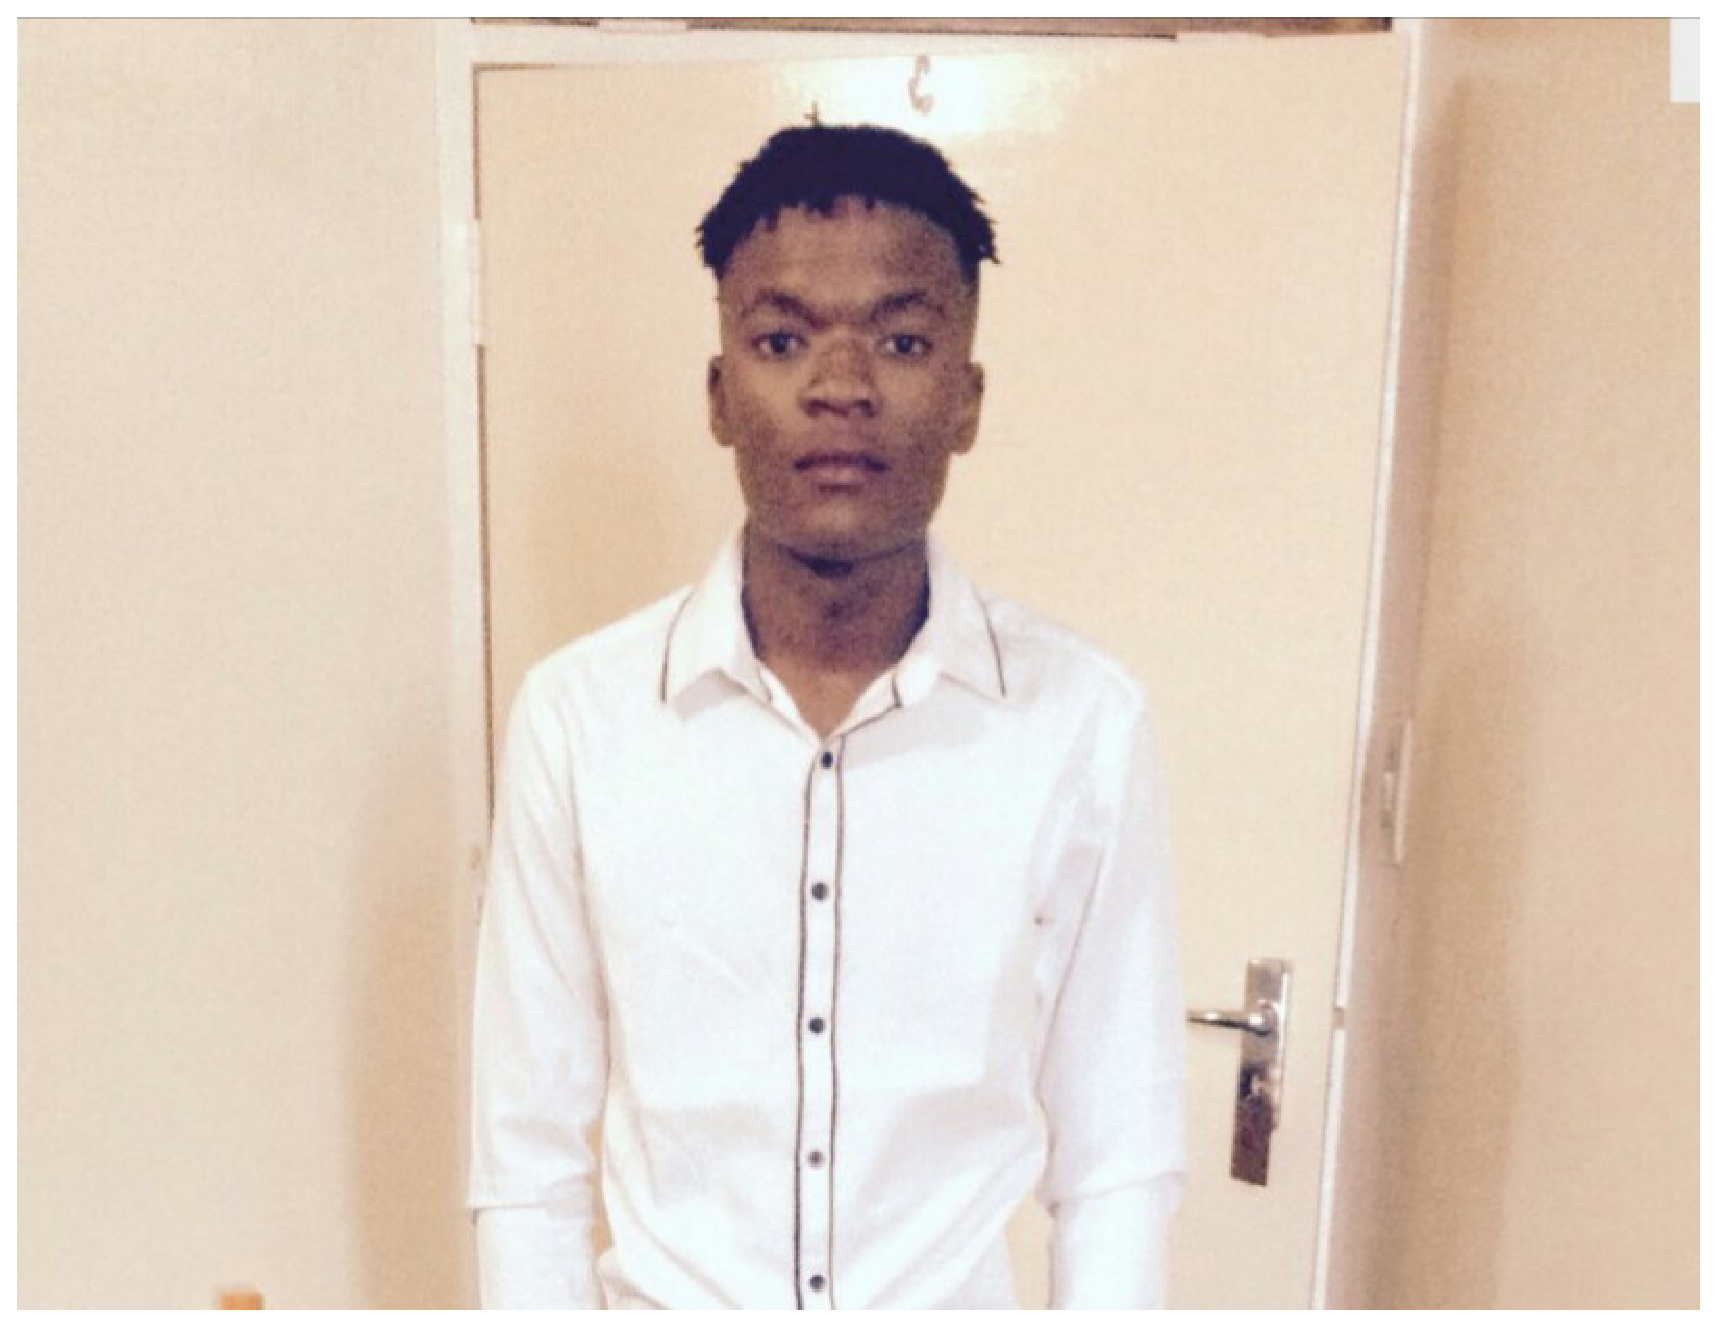
\includegraphics[width=5cm, height=5cm]{Oratile.eps} 
\end{figure}

 	\textit{. To develop 3D VR Presentation system, various interests and technical skills will be required, for example, being able to develop a system, work with different technologies and work with data analysis, also, programming skills and being able to code in multiple languages, and these are some of technical skills and interests I have listed above. Therefore, with team collaboration, and combination of common interests and skills, 3D VR Presentation system will be interesting and fun to develop.}

\begin{center}
\begin{tabularx}{1.0\textwidth}{|p{3cm}|X|}
\hline
 {\LARGE Interests} & 
 \begin{compactitem}
     \item {\large System Design}
     \item {\large Databases}
     \item {\large Software Development}
	 \item {\large System Performance}
	 \item {\large Graphics (2D and 3D)}
 \end{compactitem} \\ 
 \hline
 {\LARGE Technical Skills} & 
 \begin{compactitem}
     \item {\large Programming / Scirpting / Coding, Object-Oriented Programmming}
     \item {\large Refactoring}
     \item {\large Flexible with mutliple languages (C#, C++, Java, Mark-up Languages and Query Languages)}
 \end{compactitem} \\ 
 \hline
 {\LARGE Past Experience} & 
 \begin{compactitem}
     \item {\large Developed a CCTV system that can monitor every action at the truck weigh scale and the system is also able take screenshots at any time and store them in a database.}
 \end{compactitem} \\ 
 \hline
 {\LARGE Non-Technical Skills} & 
 \begin{compactitem}
     \item {\large Communication}
     \item {\large Collaboration}
	 \item {\large Time Management}
	 \item {\large Creativity}
 \end{compactitem} \\
 \hline 
\end{tabularx}
\end{center}
\pagebreak
% Mankgwanyane Tlaka Profile ------------------------------------------------------------------
{\huge Mankgwanyane Tlaka}
\begin{figure}[h]
\centering
\includegraphics[width=5cm, height=5cm]{Mankgwanyane.eps} 
\end{figure}

 	\textit{I want to do this project because it is very innovative, creative, challenging and my type of work}

\begin{center}
\begin{tabularx}{1.0\textwidth}{|p{3cm}|X|}
\hline
 {\LARGE Interests} & 
 \begin{compactitem}
     \item {\large Data}
     \item {\large Optimazation}
     \item {\large Software Analysis and Modelling}
 \end{compactitem} \\ 
 \hline
 {\LARGE Technical Skills} & 
 \begin{compactitem}
     \item {\large Programming} 
     \item {\large Refactoring}
     \item {\large Flexible with mutliple languages}
 \end{compactitem} \\ 
 \hline
 {\LARGE Past Experience} & 
 \begin{compactitem}
     \item {\large I worked on the Comiar Project, which required for us to design and implement a course management system.}
     \item {\large I worked on an SRC electoral Project, which allowed students of the University of Pretoria to interact with the SRC candidates.}
	 \item {\large I worked on the NavUP system under the GIS module, which  required us to gather, maintain and persist information to navigate students around campus.}
 \end{compactitem} \\ 
 \hline
 {\LARGE Non-Technical Skills} & 
 \begin{compactitem}
     \item {\large Communication}
     \item {\large Leadership}
 \end{compactitem} \\
 \hline 
\end{tabularx}
\end{center}
\pagebreak
% Tlou Lebelo Profile ----------------------------------------------------------------
{\huge Tlou Lebelo}
\begin{figure}[h]
\centering
\includegraphics[width=5cm, height=5cm]{Tlou.eps} 
\end{figure}

 	\textit{3D virtual reality among newly developed technologies is an invention of interest, not only for use but for software development.}

\begin{center}
\begin{tabularx}{1.0\textwidth}{|p{3cm}|X|}
\hline
 {\LARGE Interests} & 
 \begin{compactitem}
     \item {\large Advanced Learning in the field of Artificial Intelligence}
     \item {\large Mobile Application Software Development}
     \item {\large Using new software development tools and technologies}
 \end{compactitem} \\ 
 \hline
 {\LARGE Technical Skills} & 
 \begin{compactitem}
     \item {\large Coding (Object-Orientated Programming)} 
     \item {\large Coding(Java, C++, JavaScript, PHP}
     \item {\large Networking}
 \end{compactitem} \\ 
 \hline
 {\LARGE Past Experience} & 
 \begin{compactitem}
     \item {\large Community Based Project (JCP) - Installing computers for disadvantaged public high school in Pretoria CBD}
 \end{compactitem} \\ 
 \hline
 {\LARGE Non-Technical Skills} & 
 \begin{compactitem}
     \item {\large Team Work}
     \item {\large Good Mathematical Background}
     \item {\large Presentation Skills}
 \end{compactitem} \\
 \hline 
\end{tabularx}
\end{center}
\pagebreak
% Kenneth Mangwane Profile ------------------------------------------------------------------
{\huge Kenneth Mangwane}
\begin{figure}[h]
\centering
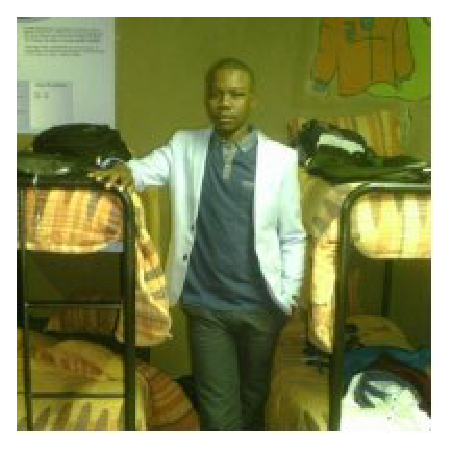
\includegraphics[width=5cm, height=5cm]{Kenneth.eps} 
\end{figure}

 	\textit{Human interaction has declined due to technology and this project will restore a large chunk on the interaction that we should have as humans.}

\begin{center}
\begin{tabularx}{1.0\textwidth}{|p{3cm}|X|}
\hline
 {\LARGE Interests} & 
 \begin{compactitem}
     \item {\large Machine Learning and Neural Networks}
     \item {\large Programming Languages}
     \item {\large Software Development}
     \item {\large Website Development}
 \end{compactitem} \\ 
 \hline
 {\LARGE Technical Skills} & 
 \begin{compactitem}
     \item {\large Programming in (C#, C, C++ and Java)} 
     \item {\large Scripting in (PHP, JavaScript and Bash)}
     \item {\large Mark-Up Language - HTML, XML, XSLT and WSDL}
     \item {\large Using Hosting Technologies and Hosting Websites}
 \end{compactitem} \\ 
 \hline
 {\LARGE Past Experience} & 
 \begin{compactitem}
     \item {\large Worked For Calibers IT Solutions as Technical and Web Designer}
     \item {\large Freelance Web Designer.}
 \end{compactitem} \\ 
 \hline
 {\LARGE Non-Technical Skills} & 
 \begin{compactitem}
     \item {\large Team work}
     \item {\large Listening}
     \item {\large Leadership}
 \end{compactitem} \\
 \hline 
\end{tabularx}
\end{center}
\pagebreak
%Team Section --------------------------------------------------------------------------
\section{Technologies: Deployment Diagram}

\section{Development Methodology}

\paragraph{The development methodology to be followed is the Agile Development Methodology. This is to allow for any changes that may be required in the development process of the system and also to minimize the risks by developing the software system in cycles called iterations.}

\paragraph{Regular team meetings will also be important in the software development process. Hence for every week, there will be three team meetings, scheduled as follows:}

\begin{itemize}
\item First meeting: Mondays
\item Second meeting: Wednesdays
\item Third meeting: Fridays
\end{itemize}

\paragraph{On Fridays, it is also important to meet with the client to discuss and give feedback about the software development process. The clients’ role will be important during the entire software development process and the role is as follows:}

\begin{itemize}
\item Frequent guidance from the client based on our process (development process).
\item -	The client should also be actively involved, this will minimize any risks of going out of the project scope.
\end{itemize}

\section{Skills and Knowledge}

\end{document}

